\documentclass[10pt,journal,compsoc]{IEEEtran}

% *** CITATION PACKAGES ***
%
\ifCLASSOPTIONcompsoc
  % The IEEE Computer Society needs nocompress option
  % requires cite.sty v4.0 or later (November 2003)
  \usepackage[nocompress]{cite}
\else
  % normal IEEE
  \usepackage{cite}
\fi
% cite.sty was written by Donald Arseneau
% V1.6 and later of IEEEtran pre-defines the format of the cite.sty package
% \cite{} output to follow that of the IEEE. Loading the cite package will
% result in citation numbers being automatically sorted and properly
% "compressed/ranged". e.g., [1], [9], [2], [7], [5], [6] without using
% cite.sty will become [1], [2], [5]--[7], [9] using cite.sty. cite.sty's
% \cite will automatically add leading space, if needed. Use cite.sty's
% noadjust option (cite.sty V3.8 and later) if you want to turn this off
% such as if a citation ever needs to be enclosed in parenthesis.
% cite.sty is already installed on most LaTeX systems. Be sure and use
% version 5.0 (2009-03-20) and later if using hyperref.sty.
% The latest version can be obtained at:
% tp://www.ctan.org/pkg/cite
% The documentation is contained in the cite.sty file itself.
%
% Note that some packages require special options to format as the Computer
% Society requires. In particular, Computer Society  papers do not use
% compressed citation ranges as is done in typical IEEE papers
% (e.g., [1]-[4]). Instead, they list every citation separately in order
% (e.g., [1], [2], [3], [4]). To get the latter we need to load the cite
% package with the nocompress option which is supported by cite.sty v4.0
% and later.



\usepackage{float}

% *** GRAPHICS RELATED PACKAGES ***
%
\ifCLASSINFOpdf
  % \usepackage[pdftex]{graphicx}
  % declare the path(s) where your graphic files are
  % \graphicspath{{../pdf/}{../jpeg/}}
  % and their extensions so you won't have to specify these with
  % every instance of \includegraphics
  % \DeclareGraphicsExtensions{.pdf,.jpeg,.png}
\else
  % or other class option (dvipsone, dvipdf, if not using dvips). graphicx
  % will default to the driver specified in the system graphics.cfg if no
  % driver is specified.
  % \usepackage[dvips]{graphicx}
  % declare the path(s) where your graphic files are
  % \graphicspath{{../eps/}}
  % and their extensions so you won't have to specify these with
  % every instance of \includegraphics
  % \DeclareGraphicsExtensions{.eps}
\fi
\usepackage{graphicx}
\graphicspath{ {./figures/} }


% NOTE: PDF hyperlink and bookmark features are not required in IEEE
%       papers and their use requires extra complexity and work.
% *** IF USING HYPERREF BE SURE AND CHANGE THE EXAMPLE PDF ***
% *** TITLE/SUBJECT/AUTHOR/KEYWORDS INFO BELOW!!           ***
\newcommand\MYhyperrefoptions{bookmarks=true,bookmarksnumbered=true,
pdfpagemode={UseOutlines},plainpages=false,pdfpagelabels=true,
colorlinks=true,linkcolor={black},citecolor={black},urlcolor={black},
pdftitle={Bare Demo of IEEEtran.cls for Computer Society Journals},%<!CHANGE!
pdfsubject={Typesetting},%<!CHANGE!
pdfauthor={Michael D. Shell},%<!CHANGE!
pdfkeywords={Computer Society, IEEEtran, journal, LaTeX, paper,
             template}}%<^!CHANGE!

\hyphenation{op-tical net-works semi-conduc-tor}


\begin{document}

\title{Experiments on Unipolar, Polar and Bipolar Line Encoding Schemes}

\author{Anudit~Nagar,~\IEEEmembership{Student,~Bennett University,}
        Abhimanyu~Banerjee,~\IEEEmembership{Student,~Bennett University}}% <-this % stops a space

\IEEEtitleabstractindextext{%
\begin{abstract}
Line encoding is a method of data transmission wherein digital data is converted to a digital signal. This paper demonstrates a platform that has been built to be utilized towards experimentation and testing for various line encoding techniques. Through this paper, common types of line encoding schemes like unipolar line encoding, polar line encoding and bipolar line encoding schemes are implemented in a virtual lab experience. Main focus of the paper is to provide a simple and optimized interface so that it can be used by people who are just starting to venture out in the field of signal encoding by providing them powerfull features built by modern development engines providing them a stable and intuitive interface to carry out experiments in a seamless manner.
\end{abstract}


\begin{IEEEkeywords}
Line Encoding Schemes, Unipolar, Polar, Bipolar, Experiments, Virtual Lab, Data Transmission, JavaScript
\end{IEEEkeywords}}

\maketitle

\IEEEdisplaynontitleabstractindextext

\IEEEpeerreviewmaketitle


\ifCLASSOPTIONcompsoc
\IEEEraisesectionheading{\section{Introduction}\label{sec:introduction}}
\else
\section{Introduction}
\label{sec:introduction}
\fi

\IEEEPARstart{C}ommunication/transmission of data from sender to receiver takes place in a computer network. Analog/digital data  traverses through communication media from source to destination in form of signals.The transmitting signals may undergo attenuation and distortion as they travel over large distances.Therefore there is a need to match the properties of transmitted signal as per the communication media for which digital data can be converted into digital signals. This conversion or encoding techniques is what will be covered in this paper.


Line encoding: The process of converting digital data into digital signals is referred as Line Encoding.With the help of line encoding schemes, a sequence of bits are converted into digital signal(encoding) which then get converted back into bits at the receiver end (decoding).

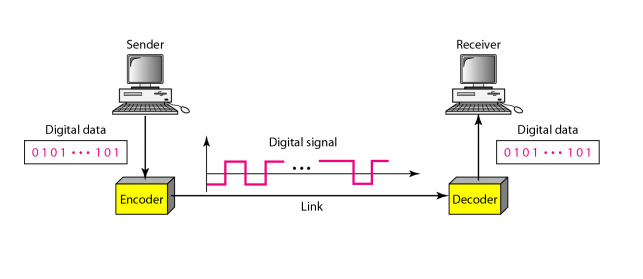
\includegraphics[scale=0.37]{figures/intro1.png}

\subsection{Signal Transmission Issues}
Dc components: After line coding has been applied onto the data to be transmitted, their is a possibility of the signal having a zero frequency component in the transmitted signal which is called DC component. This DC component in the spectrum (caused due to constant voltage level in digital signal) is unable to pass through communication medium components like transformers due to which distortion of transmitting signal takes place.


Self Synchronization: The bit interval of the receiver and that of the transmitter must be synchronized  inorder to correctly interpret the received signal. If the clock at the receiver end is faster or slower, the bit intervals will not match and misinterpretation of received signal will take place.


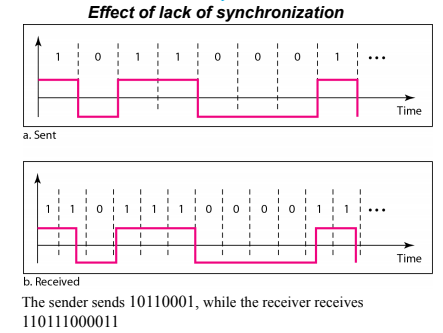
\includegraphics[scale=0.5]{figures/intro2.png}

\section{Literature Review/Related Work}
We worked on analysing previous techniques of signal visualisation experiments and the techniques they utilized to visualize and implement the experimentation details. This sheds light towards a deeper understanding of signal encoding technologies and the related optimisations offered in these papers. A brief overview of our leanings from these are further discussed below.

\subsection{SYNTHESIS AND SIMULATION OF AMI AND MANCHESTER CODING USING VHDL LANGAUGE}
This is a research paper by Garima Saraf, Prerna Gupta and MD. Zahid Alam which is a demonstration of Encoding schemes. The techniques to be implemented are selected based on the systems performance criteria.Signal to noise ratio for longer and shorter signals has been studied in this paper based on which data coding techniques to be implemented are selected. Also various other factors like error checking have been taken into account.

\subsection{Blind Classification of Line-Coding Schemes Based on Characteristic Features}
This is a research paper published in the IEEE stating the implementation and use of line encoding techniques in modern defence systems.Signalling technologies are a key component of military operations, for which line encoding techniques has been explored in this paper.Characteristic features of digital data to digital signals techniques have been examined in this paper based on which a blind classification algorithms has been proposed.   

\subsection{Method of Unipolar Digital to Digital Encoding Data Transmission}
Method of Unipolar Digital to Digital Encoding Data Transmission
This is a published paper by Nuha Abdelmageed and Jabar Alzubaidi which proposes data transmission  via unipolar encoding schemes. The paper talks about various other common types of line encoding methods. The hardware implementation using latch SN74373, amplifier  ULN 2003-500 mA and C++ language has been represented in the paper.  

\subsection{Design of Manchester Digital to Digital Encoding Data Transmission}
A detailed analysis of Biphase encoding techniques like Manchester and their advantages over other digital data to digital signal transmission schemes have been covered in this paper. This paper mentions both software and hardware implementation of the research topic.This paper specifically concludes with three reasons why biphase techniques have an edge over other techniques which includes modulation rate,synchronization and error detection as key factors of comparison
Data Resources

\section{Technological Resources Used}

\subsection{Visual Representation}
Our platform uses Plotly.js. It is a high level, declarative plotting library written in JavaScript. Plotly charts are described as JSON objects which are imported in our project. All aspects of the charts like colors, lines, legends have a corresponding set of attributes which can be controlled by the developer. Graphs with Plotly are drawn as Scalar Vector Graphics offering great compatibility across browsers and platforms along with vector image exports. Plotly internally uses Stack.Gl for high -performance multi-dimensional charting.

\subsection{Project Stack}
Our platform utlizes HTML as the markup language that to structure and give meaning to our web content.
Cascading Style Sheets is a language of style rules that we use to apply styling to our Structured Markup content.
JavaScript is a scripting language that enables us to create dynamically updating content, control graphs, animate text and images.
JSON (JavaScript Object Notation) based unit

\subsection{Deployment Strategy}
We use a serverless infrastructure for the deployment of our project which is used to publish new builds of the platform directly using our Continuous Integration and Continuous Deployment (CICD) build pipeline. This eliminated the need to maintain physical infrastructure, systems and software from the developer's standpoint. Serverless architectures allows us to build  highly scalable experimentation platforms, delivering high performance and seamless experienced to the developers and the users of the platform.

\section{Methodology}

Polar encoding comprises of two levels of positive and negative of amplitude. Types of Polar encoding techniques are:                   

Types of encoding are: 
\begin{itemize}
    \item Unipolar
        \begin{itemize}
             \item Return to Zero (RZ)
           \end{itemize}
     \item Polar
     \begin{itemize}
      \item Non Return to Zero(NRZ)
           \begin{itemize}
             \item NRZ-L
             \item NRZ-I
           \end{itemize}
      \item Bi Phase
           \begin{itemize}
             \item Manchester
             \item Differential Manchester
           \end{itemize}
    \end{itemize}
    \item Bipolar
           \begin{itemize}
             \item AMI
             \item Pseudoternary
           \end{itemize}
\end{itemize}



\subsection{Setup}
When the user starts the application, they are presented with a central dashboard with various experiments listed that are available to perform. Here they can choose whichever encoding scheme they would like to experiment with and the application will take them to a dedicated space where the experiments for that specific encoding can be carried out.

\begin{figure}[h]
\centering
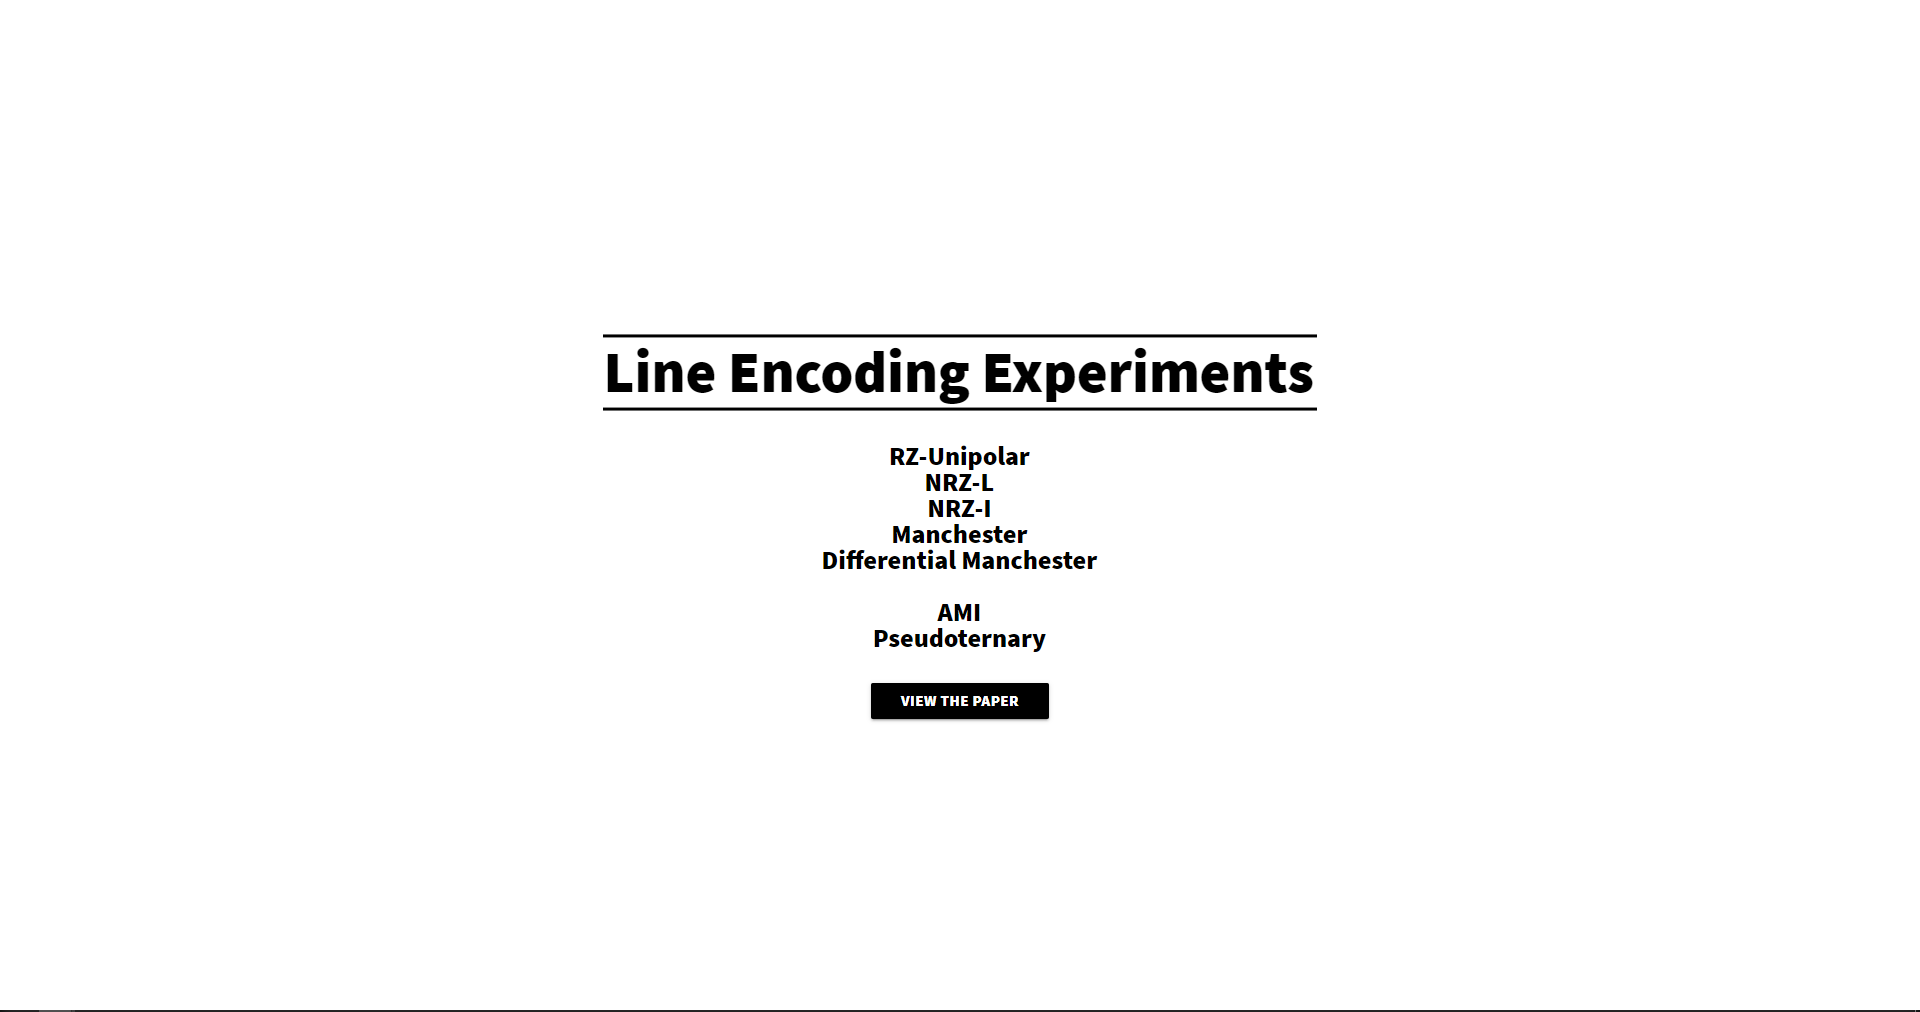
\includegraphics[scale=0.15]{one.png}
\caption{Image of Dashboard}
\end{figure}

\begin{figure}[H]
\centering
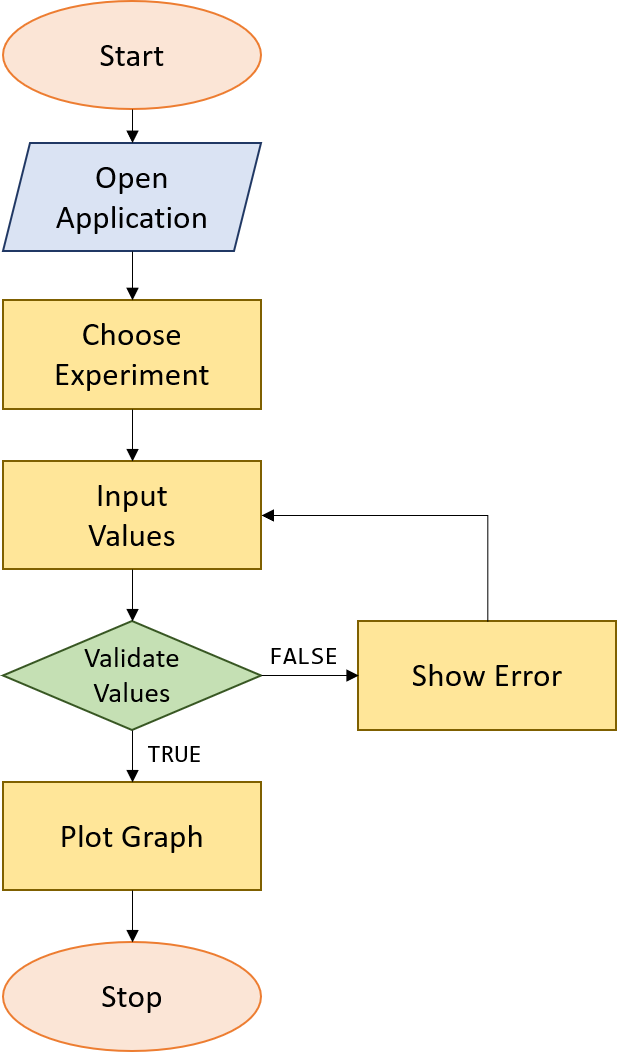
\includegraphics[scale=0.5]{flowchart.png}
\caption{Flow of Project}
\end{figure}

\subsection{Unipolar RZ (Return to Zero)}
In this scheme binary 1  is represented with a high voltage in first half of the bit and in the other half it returns to zero whereas 0 bit is simply represented by 0 level . You can refer to the figure below for a better understanding of the encoding scheme.

\begin{figure}[H]
\centering
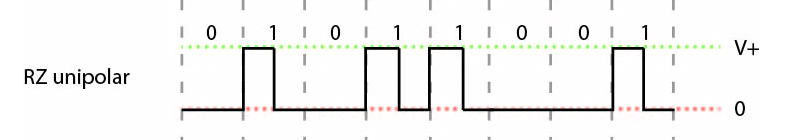
\includegraphics[scale=0.35]{encoding-rz.png}
\caption{RZ Encoding}
\end{figure}

\subsection{NRZ-I (Non Return to Zero -Invert)}
For logical 1 the signal will be inverted, but when it encounters logical 0 then signal will not undergo any transition. This is the NRZ-Invert. You can refer to the figure below for a better understanding of the encoding scheme.

\begin{figure}[H]
\centering
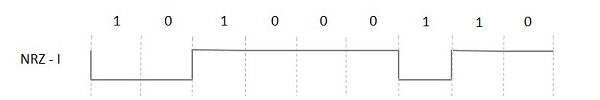
\includegraphics[scale=0.55]{encoding-nrzi.png}
\caption{NRZ-I Encoding}
\end{figure}


\subsection{NRZ-L (Non Return to Zero -Level)}
In NRZ-L type of encoding, high volt is assigned for logical 0 bit and low volt is assigned for logical 1. Level of voltage determines bit value. This is NRZ-Level. You can refer to the figure below for a better understanding of the encoding scheme.


\begin{figure}[H]
\centering
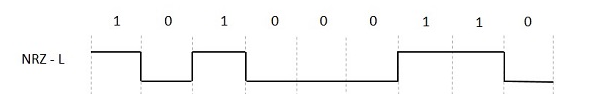
\includegraphics[scale=0.55]{encoding-nrzl.png}
\caption{NRZ-l Encoding}
\end{figure}


\subsection{Manchester}
It is a combination of NRZ-L and RZ. The duration of each bit is divided into two halves. 0 is \raisebox{0pt}{\fbox{
\includegraphics[height=6pt]{signal1.png}}} and 1 is \raisebox{0pt}{\fbox{
\includegraphics[height=6pt]{signal2.png}}}. You can refer to the figure below for a better understanding of the encoding scheme.

\begin{figure}[H]
\centering
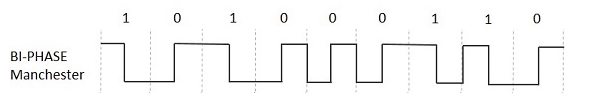
\includegraphics[scale=0.55]{encoding-manchester.png}
\caption{Manchester Encoding}
\end{figure}


\subsection{Differential Manchester}
It combines the idea of RZ and NRZ-I.If the next bit is 0,transition will occur but if the next bit is 1 , no transition will occur. You can refer to the figure below for a better understanding of the encoding scheme.

\begin{figure}[H]
\centering
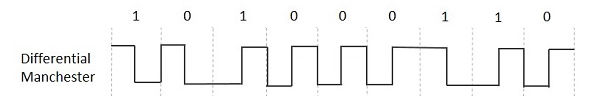
\includegraphics[scale=0.55]{encoding-diffmanchester.png}
\caption{Differential Manchester Encoding}
\end{figure}



\subsection{AMI}
In Alternate Mark Inversion or AMI, 0 bit is represented by Zero level and binary 1 is represented by alternating positive and negative voltages. You can refer to the figure below for a better understanding of the encoding scheme.

\begin{figure}[H]
\centering
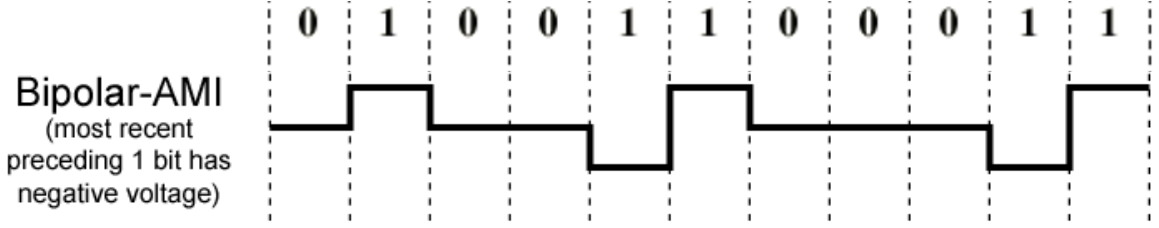
\includegraphics[scale=0.25]{encoding-ami.png}
\caption{AMI Encoding}
\end{figure}


\subsection{Pseudoternary}
Pseudoternary is similar to AMI with slight difference that alternating positive and negative is used for binary 0 instead of binary 1. You can refer to the figure below for a better understanding of the encoding scheme.

\begin{figure}[H]
\centering
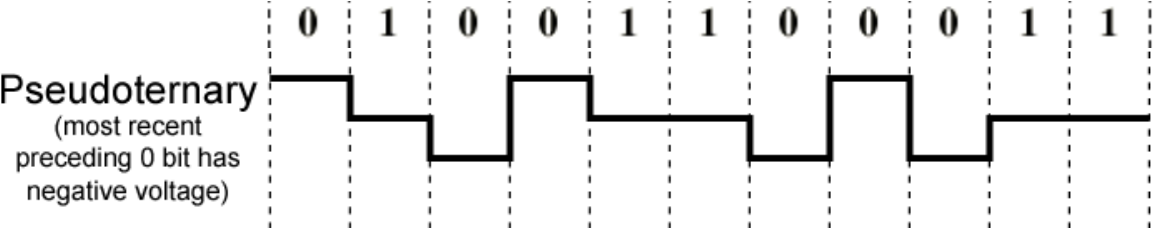
\includegraphics[scale=0.25]{encoding-pseudoternary.png}
\caption{Pseudoternary Encoding}
\end{figure}

\section{Results}

Input for the following tests is 10101.

\subsection{Unipolar RZ }

In the result below as we incur a 1 there is high voltage in first half of the bit and zero level in second half. Whereas when it is a 0 bit signal remains at zero level. 

\begin{figure}[H]
\centering
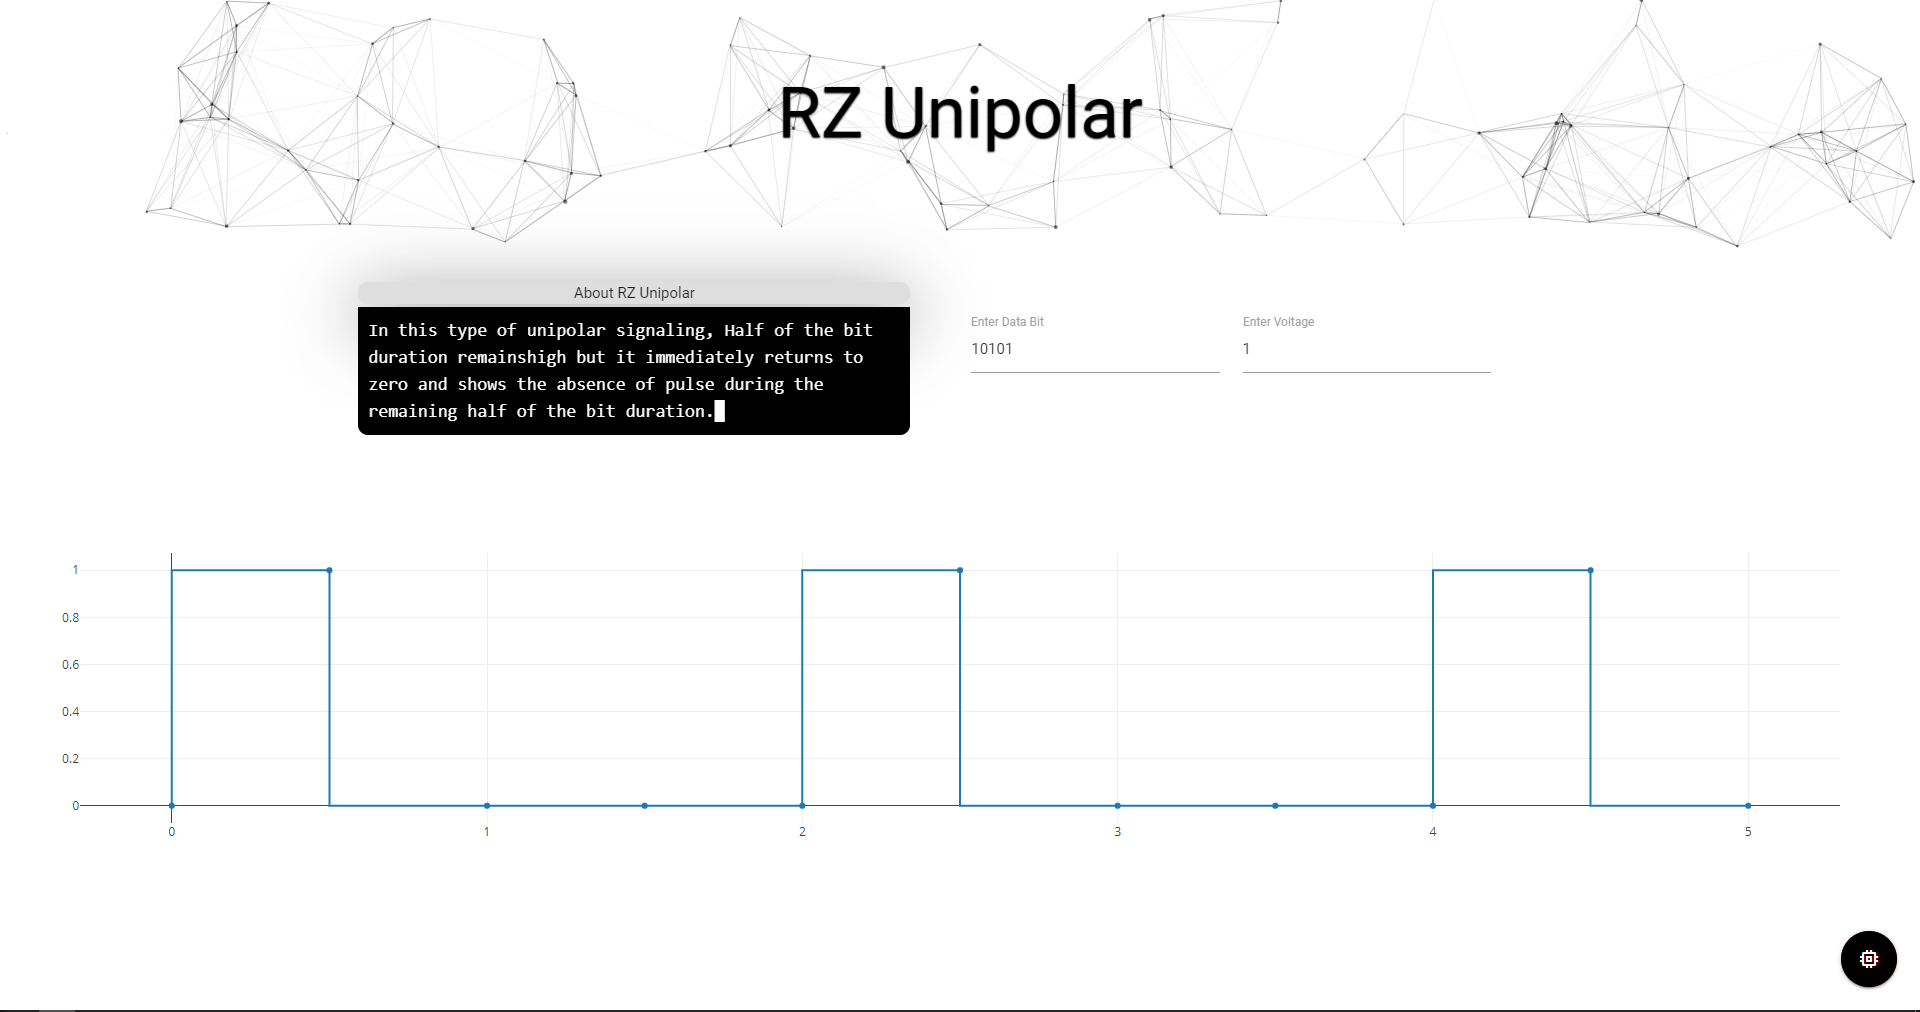
\includegraphics[scale=0.15]{rz.png}
\caption{RZ Experiment Dashboard}
\end{figure}

\subsection{NRZ-I }

Starting with low voltage for 1 then next bit is 0 so no inversion. Then inversion takes place as next bit is 1 and remains same as next come 0. Again there is an inversion as next bit is 1.

\begin{figure}[H]
\centering
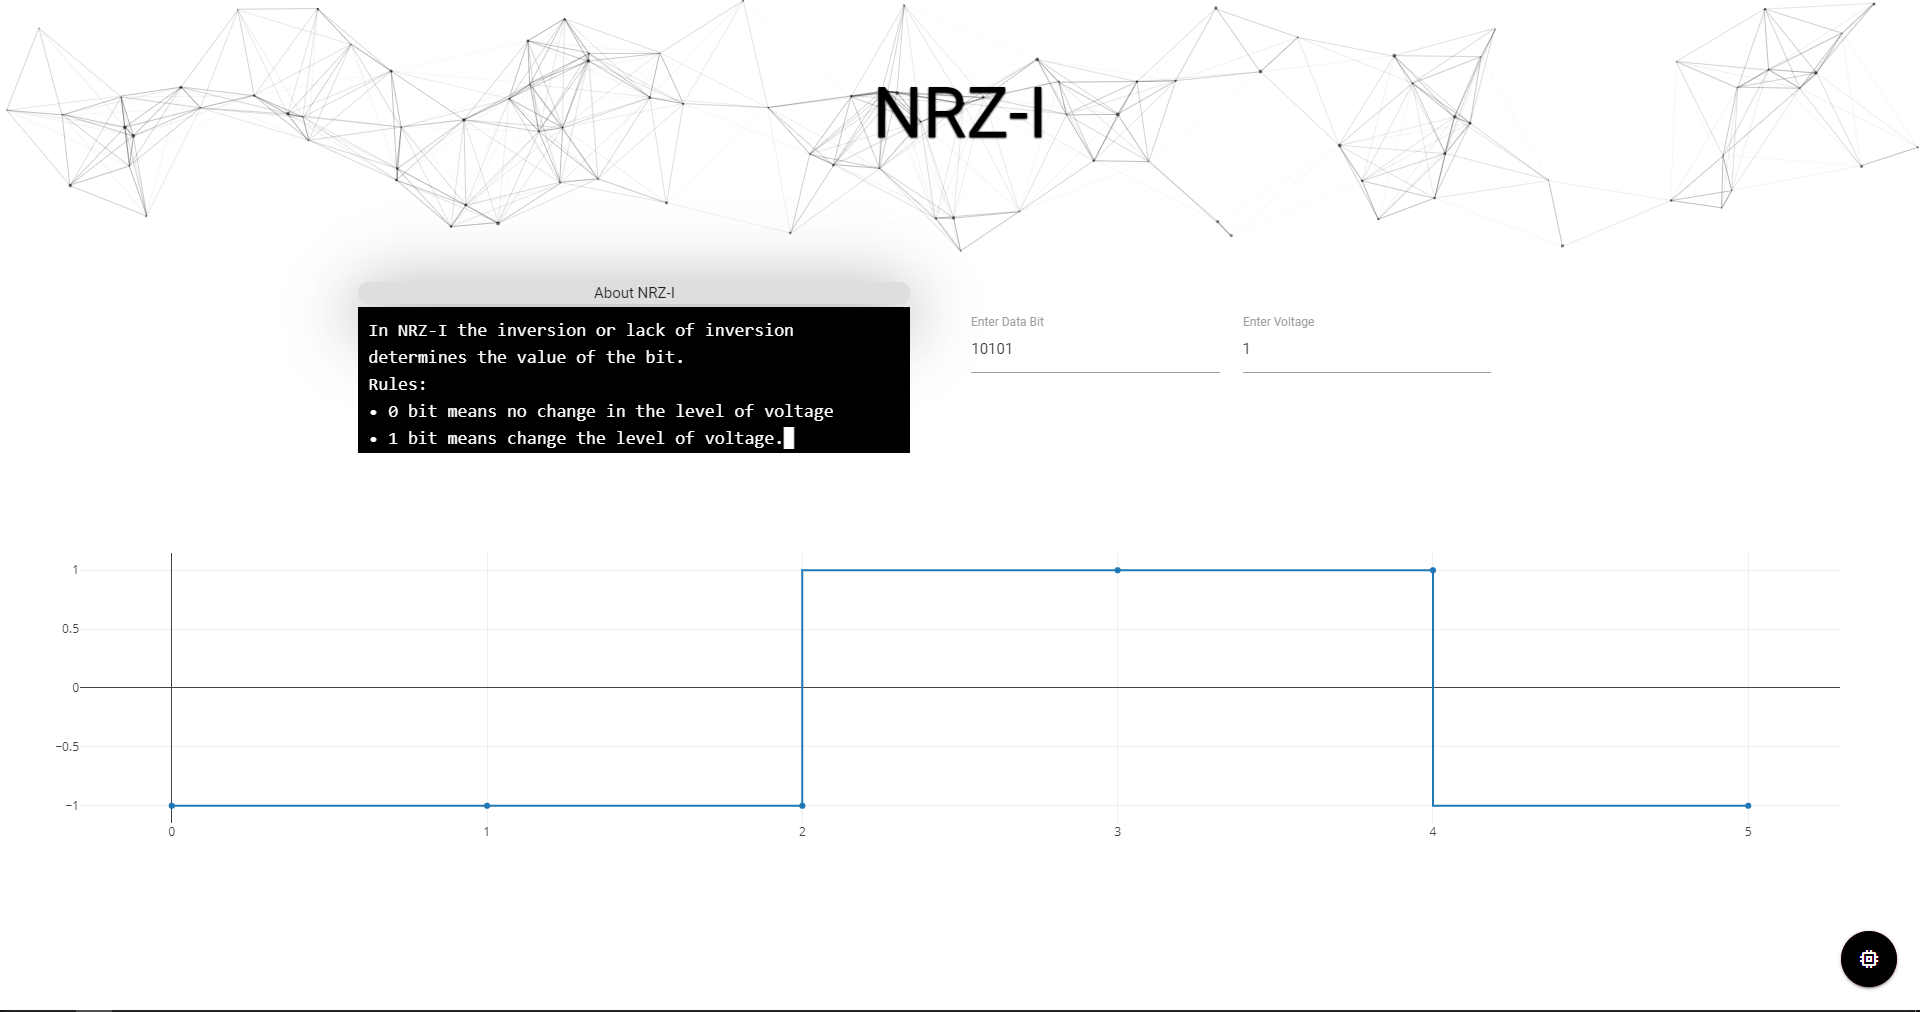
\includegraphics[scale=0.15]{nrzi.png}
\caption{NRZI Experiment Dashboard}
\end{figure}

\subsection{NRZ-L}

When we incur  0 in sequence of bits high voltage is set and when 1 comes low voltage is set.

\begin{figure}[H]
\centering
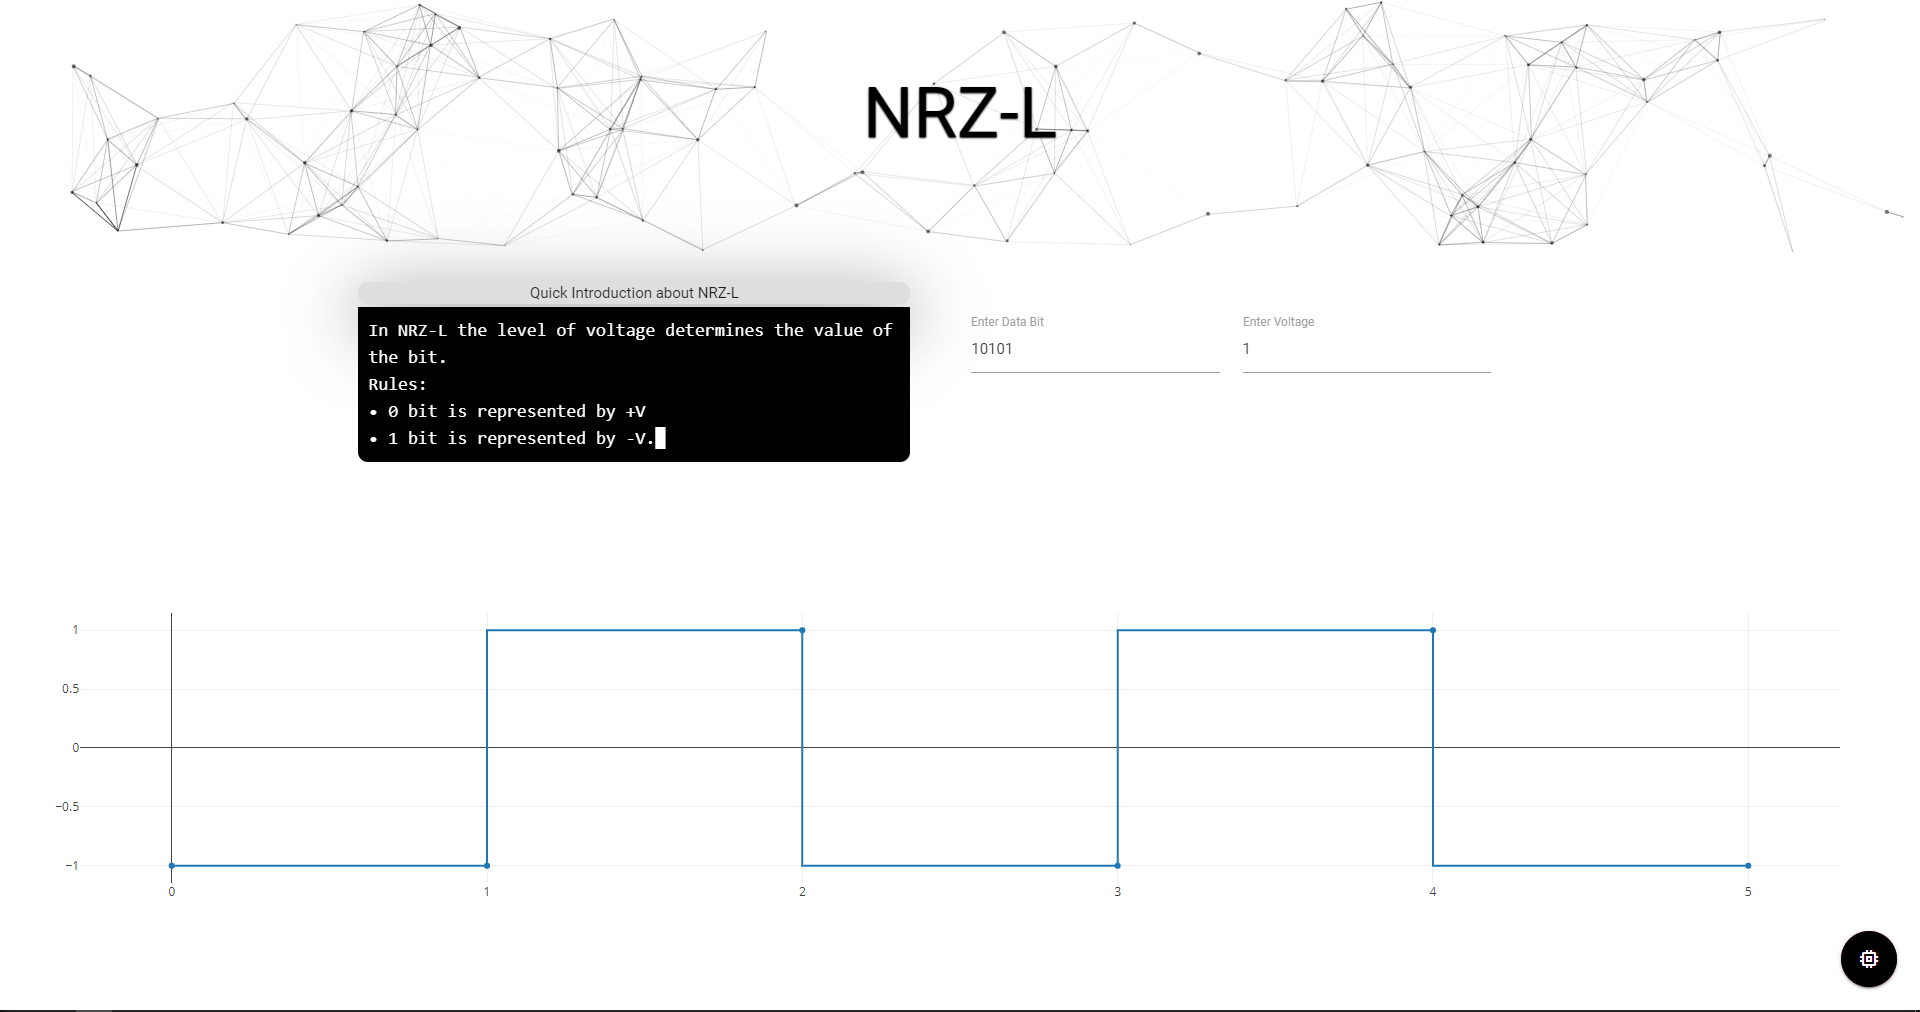
\includegraphics[scale=0.15]{nrzl.png}
\caption{NRZL Experiment Dashboard}
\end{figure}


\subsection{Manchester}

As we get a 0 we set a \raisebox{0pt}{\fbox{
\includegraphics[height=6pt]{signal1.png}}} in the signal and a \raisebox{0pt}{\fbox{
\includegraphics[height=6pt]{signal2.png}}} when there is 1 is the sequence of bits.


\begin{figure}[H]
\centering
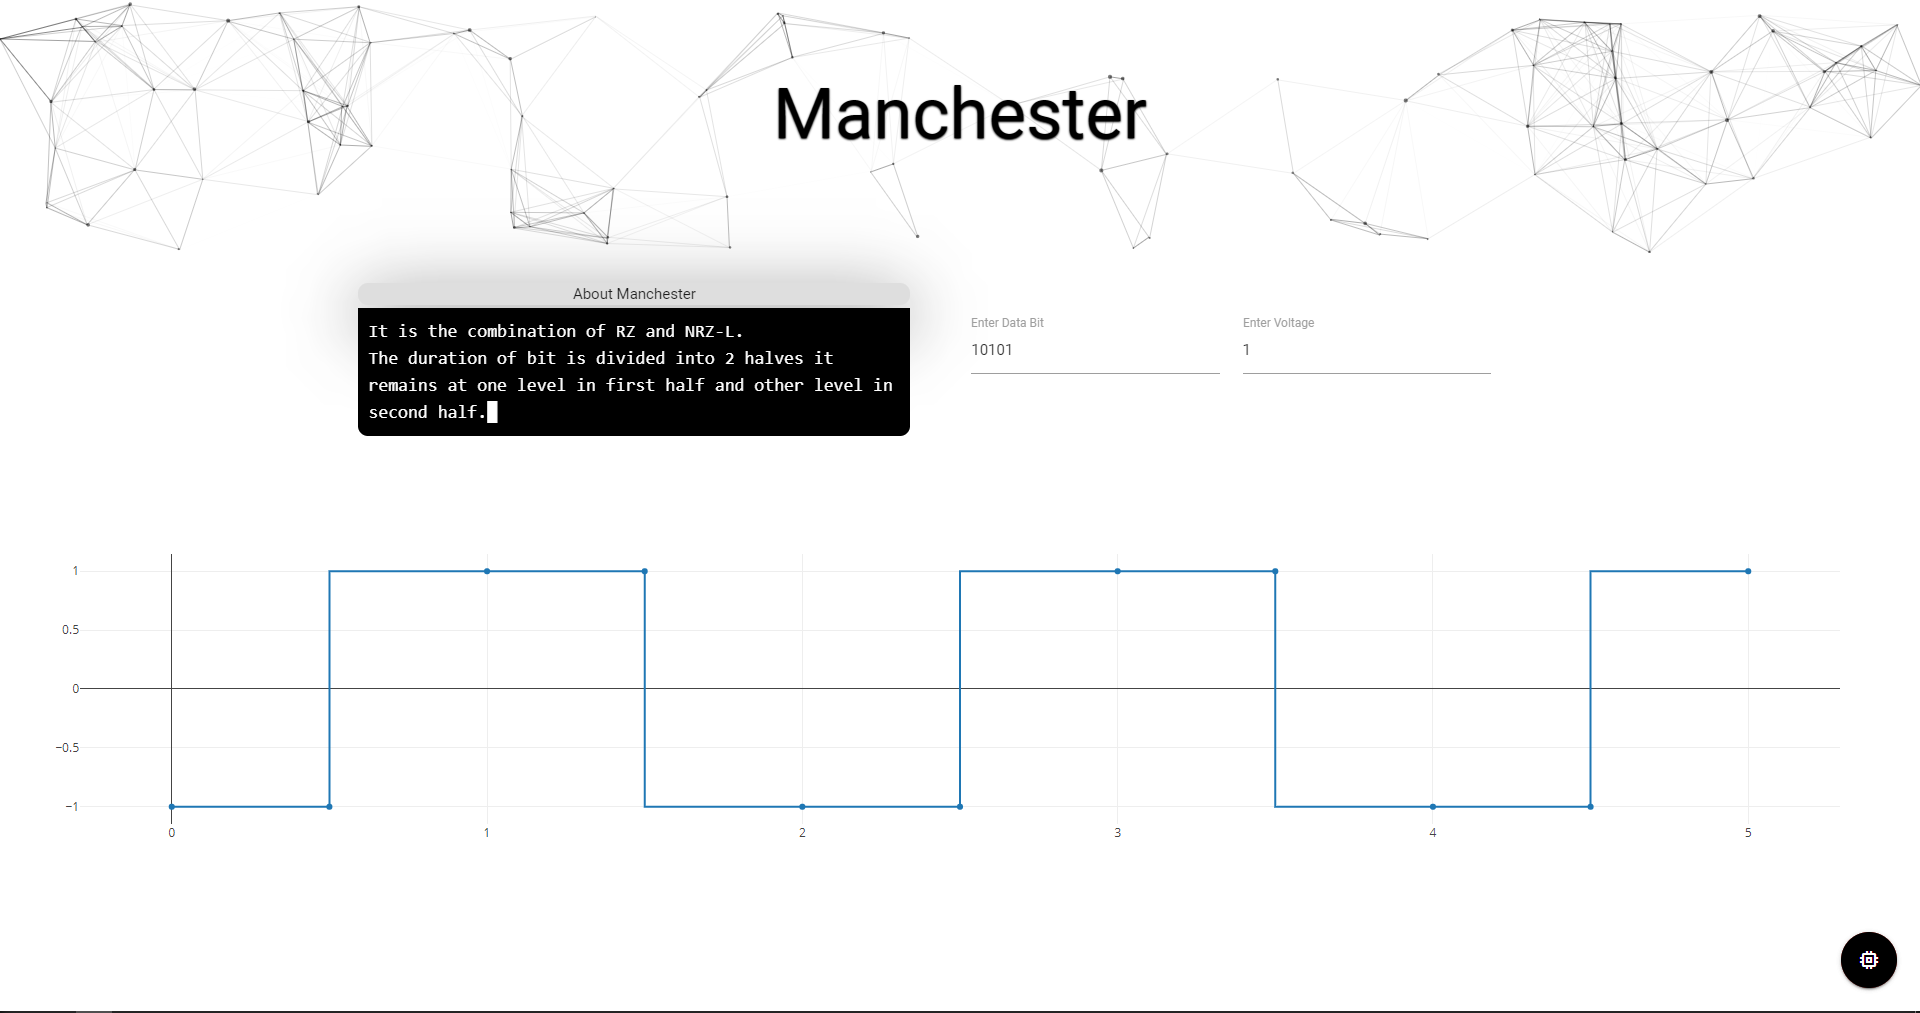
\includegraphics[scale=0.15]{manchester.png}
\caption{Manchester Experiment Dashboard}
\end{figure}

\subsection{Differential Manchester}

 First we set the depicted signal for 1 then next is 0 for which we have an inversion. As next bit is 1 so there would be no inversion taking place and so on.

\begin{figure}[H]
\centering
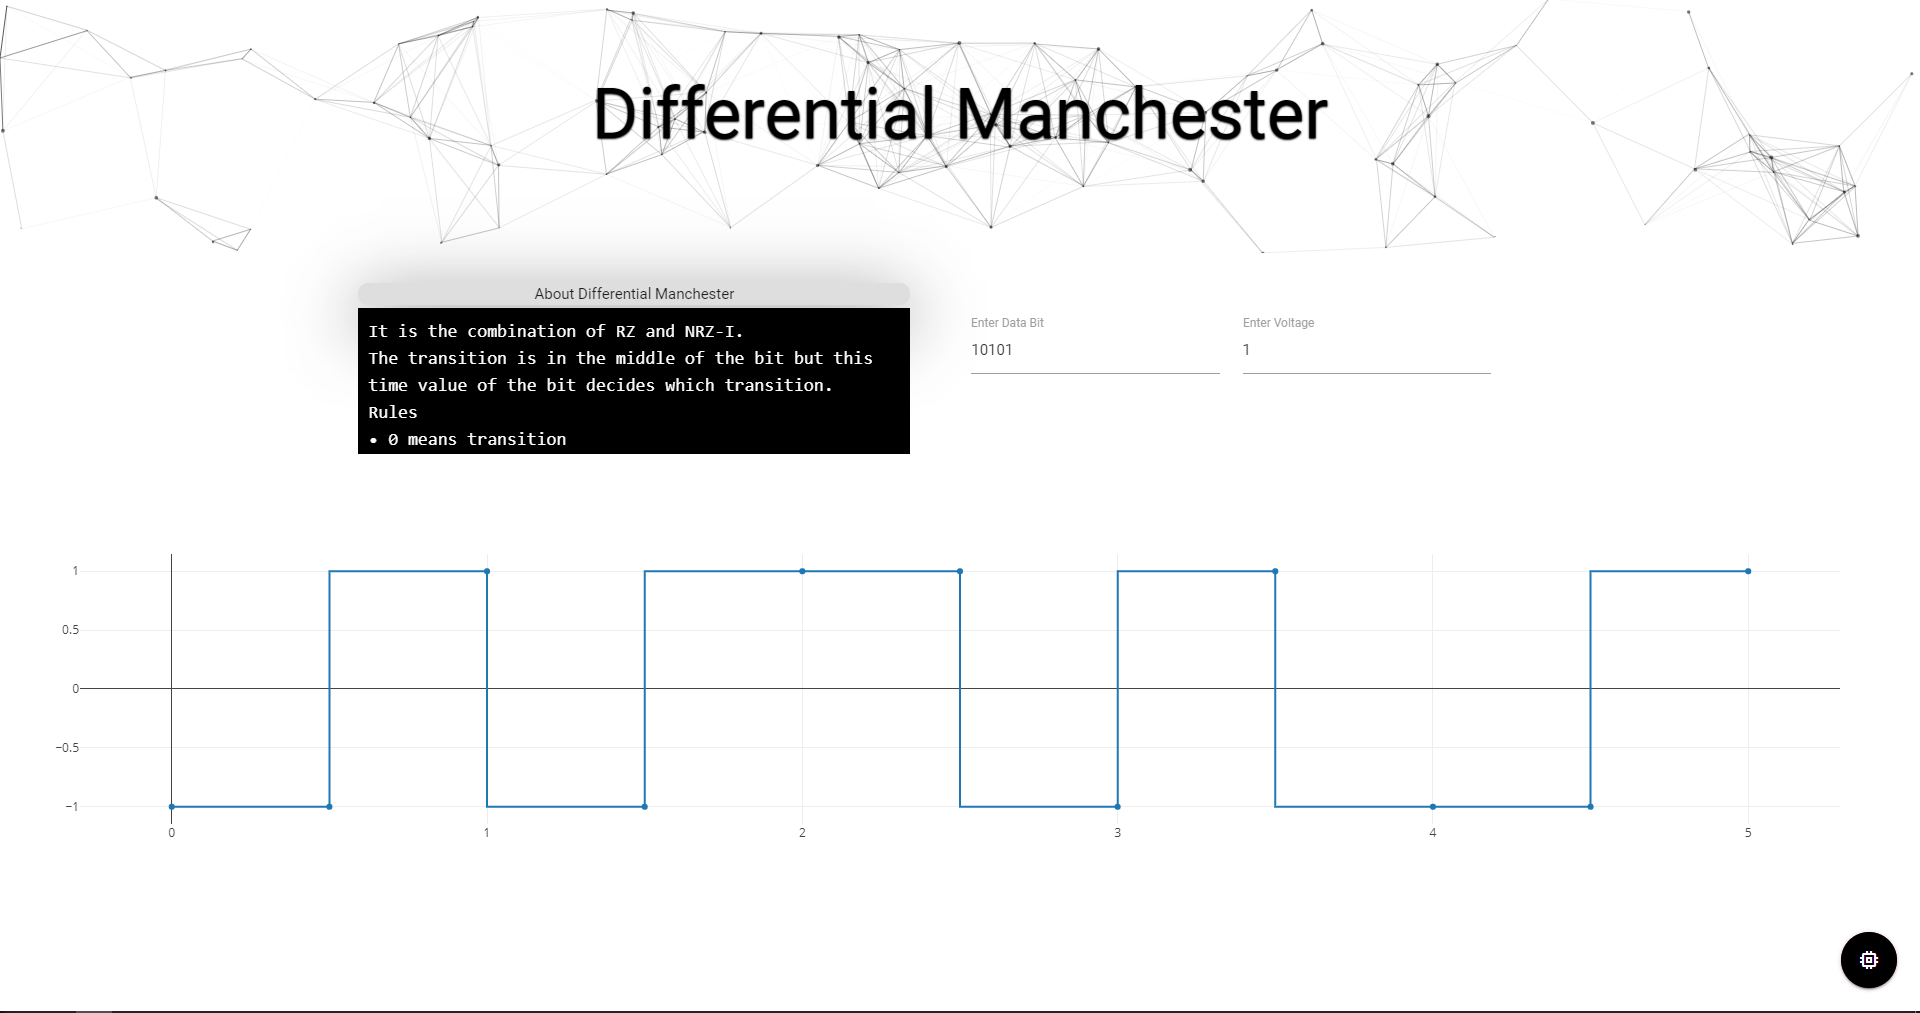
\includegraphics[scale=0.15]{diffmanchester.png}
\caption{Differential Manchester Experiment Dashboard}
\end{figure}


\subsection{AMI}

For first 1 we set positive high voltage and then for zero we set zero level.But for next one we will set a voltage opposite to that of the previous 1 therefore we set  negative voltage and the same alternating pattern is applied further when there is a 1 in the sequence.

\begin{figure}[H]
\centering
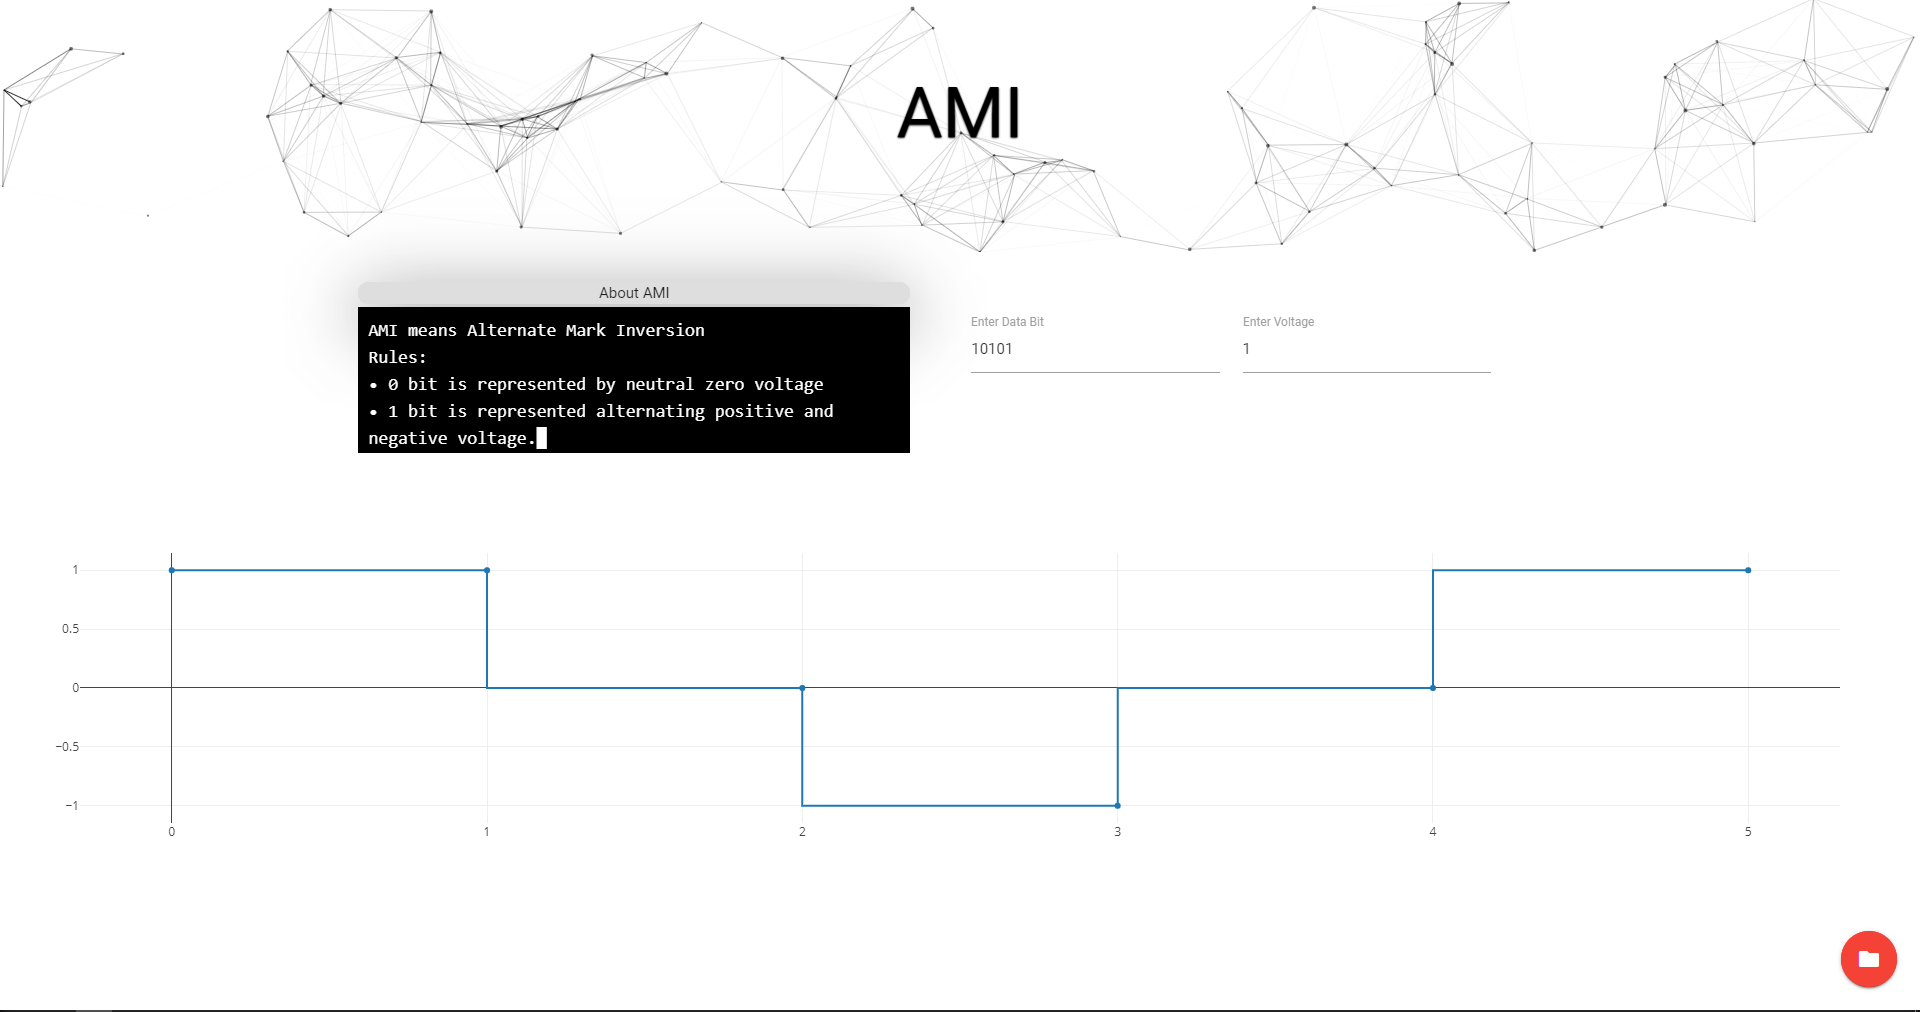
\includegraphics[scale=0.15]{AMI.png}
\caption{AMI Experiment Dashboard}
\end{figure}


\subsection{PSEUDOTERNARY}

The resulting signal is generated similarly like in the case of AMI except zero level is set for 1 bit and the alternating pattern is applied for 0 bit.

\begin{figure}[H]
\centering
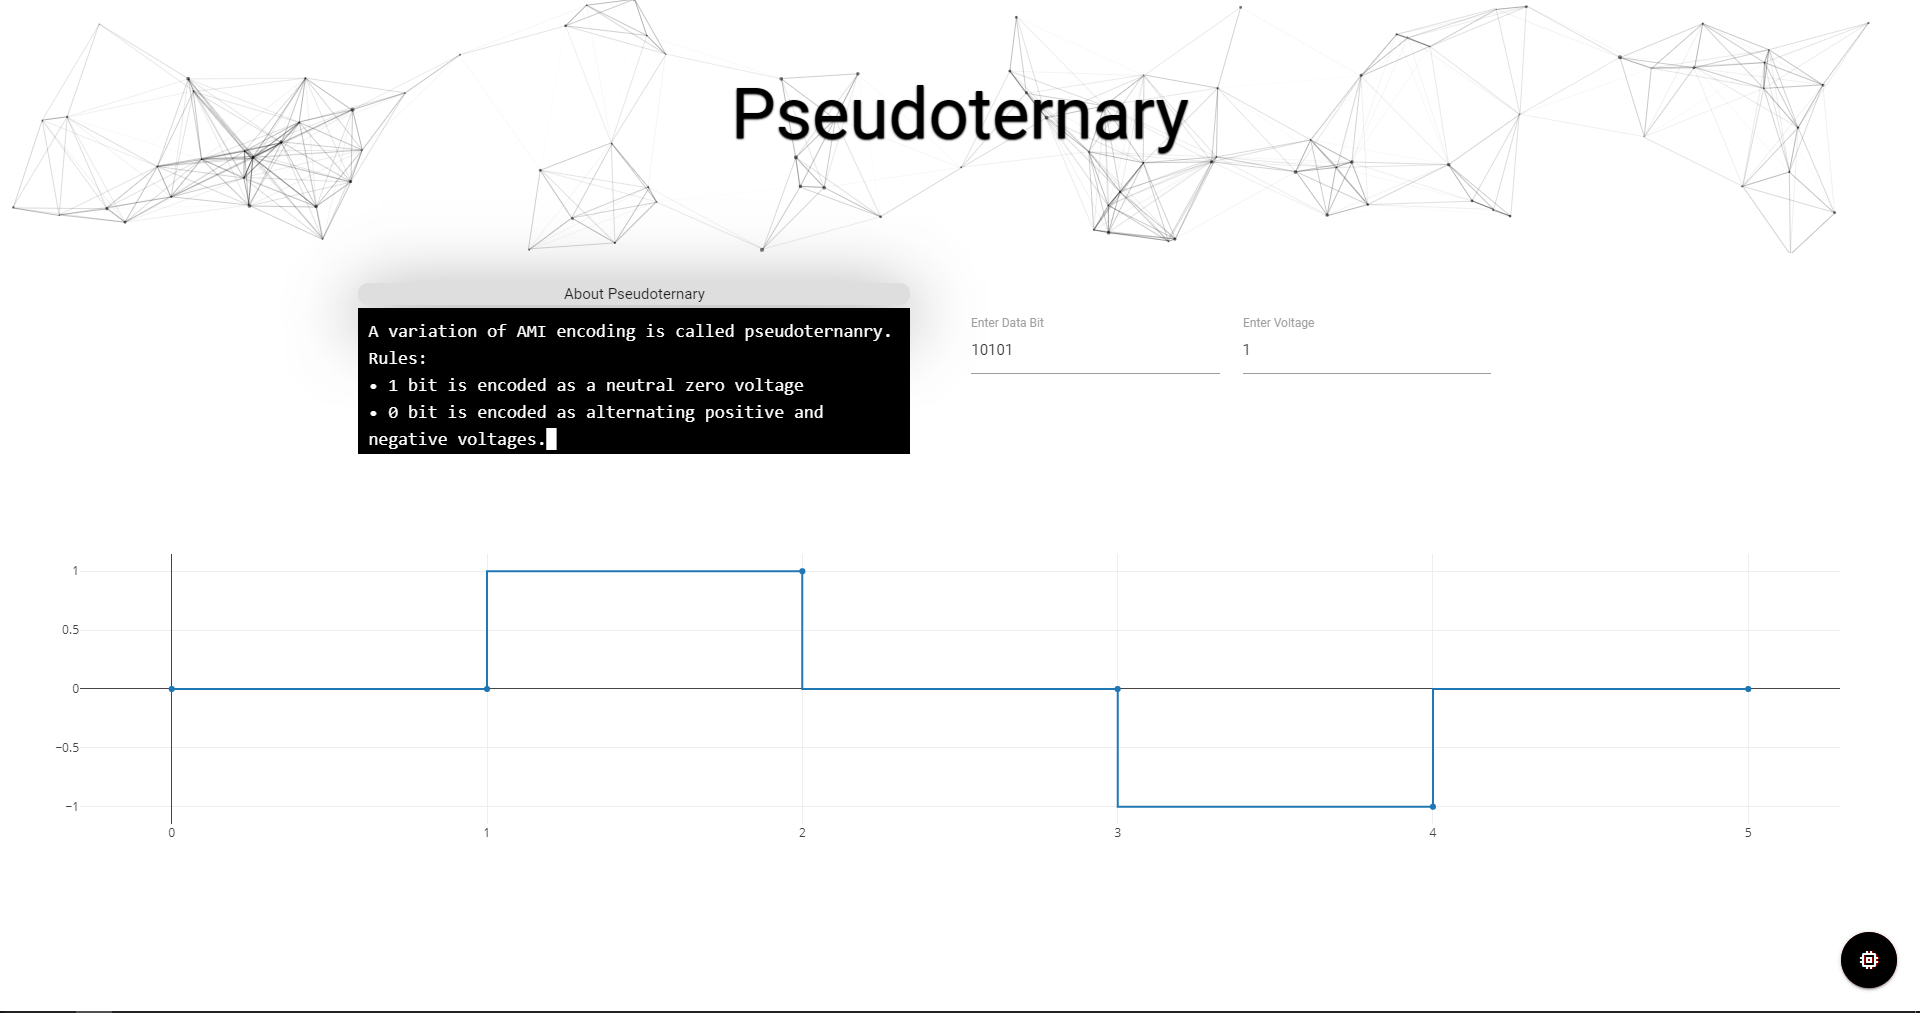
\includegraphics[scale=0.15]{pseudoternary.png}
\caption{PSEUDOTERNARY Experiment Dashboard}
\end{figure}

\subsection{Contributions}

Our experimentation platform shows massive performance improvements and cross platform compatibility allowing anyone with an internet connection to perform experiments online using a virtual lab experience. It removes the hassle of installing dependencies and configuring a development environment making the platform accessible to everyone. It offers advanced features like live updates and in-browser voltage control while keeping the interface simple and optimized so that it can be used by people who are just starting to venture out in the field of signal encoding.

\section{Conclusion}
This project showcase an advanced mechanism for line encoding experimentation. It brings features like cross-platform compatibility, live-updates, dynamic voltage control, modern plotting libraries with granular control of generated graphs and the ability to save results for future use. These advanced features are presented in a simplistic manner to make them simple and accessible by everyone. The platform takes the leanings from various previous works and creates a culmination of these to offer a modern experimentation platform that is available virtually.

% use section* for acknowledgment
\ifCLASSOPTIONcompsoc
  % The Computer Society usually uses the plural form
  \section*{Acknowledgments}
\else
  % regular IEEE prefers the singular form
  \section*{Acknowledgment}
\fi

We would like to express our special thanks and gratitude to our Computer Network professor Dr. Kuldeep Chaurasia and Dr. Vijay Bohat for their able support and guidance to complete this project.  

\ifCLASSOPTIONcaptionsoff
  \newpage
\fi

\begin{thebibliography}{1}

\bibitem{IEEEhowto:kopka}
H.~Kopka and P.~W. Daly, \emph{A Guide to {\LaTeX}}, 3rd~ed.\hskip 1em plus
  0.5em minus 0.4em\relax Harlow, England: Addison-Wesley, 1999.
  
\bibitem{bjdmn264}
Garima Saraf and Prerna Gupta and Md. Alam, \emph{Synthesis and simulation of AMI and Manchester coding using VHDL Langauge}, Binary Journal of Data Mining I\& Networking, 2012

\bibitem{7934310}
J. {Oh} and J. {Jeong} and Y. {Jang} and J. {Lee} and D. {Yoon}, \emph{Blind Classification of Line-Coding Schemes Based on Characteristic Features}, IEEE Access , 2017

\bibitem{4}
Amna Mohammed Elzain,Abdelrasoul Jabar Alzubaidi, \emph{Method of Unipolar Digital to Digital Encoding Data Transmission}, IOSRJEN, 2014

\bibitem{5}
Amna Mohammed Elzain,Abdelrasoul Jabar Alzubaidi, \emph{Design of Manchester Digital to Digital Encoding Data Transmission}, IOSRJEN, 2015

\end{thebibliography}

\end{document}


